\documentclass[tikz, margin=3.14mm]{standalone}
\usetikzlibrary{backgrounds}

\begin{document}
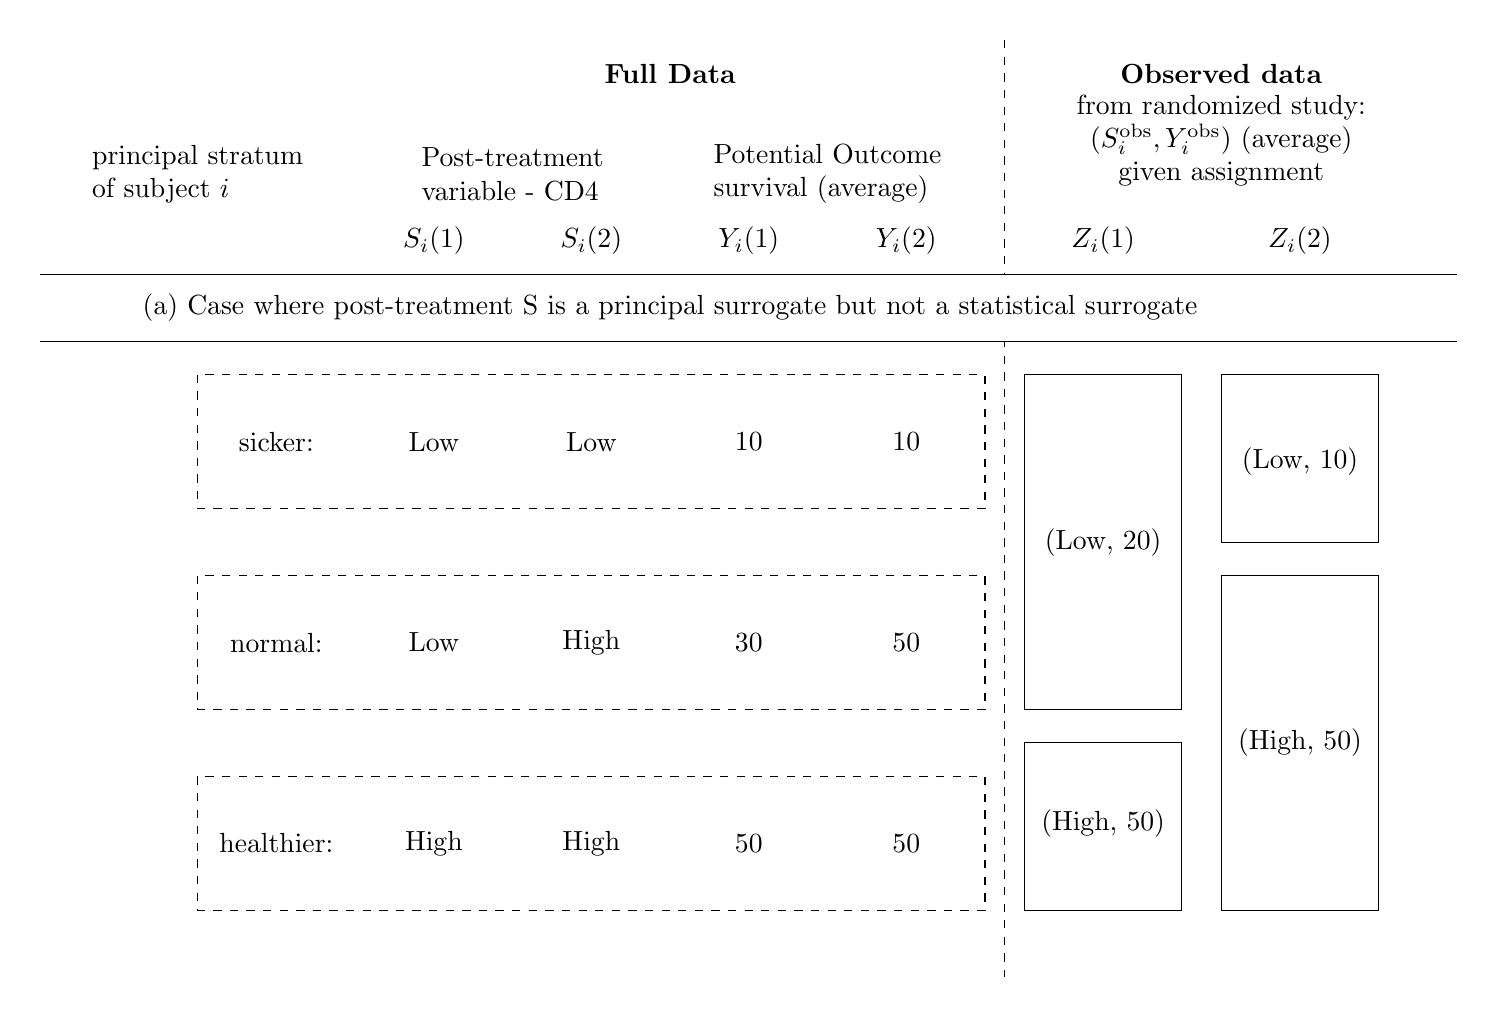
\begin{tikzpicture}[scale=2, yscale=.85, every node/.style={align=left}, 
    background rectangle/.style={fill=white}, show background rectangle]

% nodes --- 
\node at (0,0) {principal stratum \\ of subject $i$};
\node at (2,0) {Post-treatment \\ variable - CD4};
\node at (4,0) {Potential Outcome \\ survival (average)};
\node at (1.5,-.5) {$S_i(1)$};
\node at (2.5,-.5) {$S_i(2)$};
\node at (3.5,-.5) {$Y_i(1)$};
\node at (4.5,-.5) {$Y_i(2)$};

\node at (3, .75) {\textbf{Full Data}};

\draw [dashed] (5.125, 1) -- (5.125, -6);
\filldraw [draw=none, fill=white] (-1,-.75) rectangle (8,-1.25);
\node at (3,-1) [align=center] {(a) Case where post-treatment S is a principal surrogate but not a statistical surrogate};
\node [align=center] at (6.5, 0.75) {\textbf{Observed data}};
\node [align=center] at (6.5, 0.25) {from randomized study: \\ $(S_i^{\mathrm{obs}}, Y_i^{\mathrm{obs}})$ (average) \\ given assignment};

\node at (5.75,-.5) {$Z_i(1)$};
\node at (7,-.5) {$Z_i(2)$};

\draw (-1,-.75) to (8, -.75);
\draw (-1,-1.25) to (8, -1.25);


\filldraw [dashed, fill=none] (0, -1.5) rectangle (5, -2.5);
\filldraw [dashed, fill=none] (0, -3) rectangle (5, -4);
\filldraw [dashed, fill=none] (0, -4.5) rectangle (5, -5.5);

\node at (.5, -2) {sicker:};
\node at (.5, -3.5) {normal:};
\node at (.5, -5) {healthier:};

\node at (1.5, -2) {Low};
\node at (2.5, -2) {Low};
\node at (3.5, -2) {10};
\node at (4.5, -2) {10};

\node at (1.5, -3.5) {Low};
\node at (2.5, -3.5) {High};
\node at (3.5, -3.5) {30};
\node at (4.5, -3.5) {50};

\node at (1.5, -5) {High};
\node at (2.5, -5) {High};
\node at (3.5, -5) {50};
\node at (4.5, -5) {50};

\draw (5.25, -1.5) rectangle (6.25, -4);
\node at (5.75, -2.75) {(Low, 20)};

\draw (5.25, -4.25) rectangle (6.25, -5.5);
\node at (5.75, -4.85) {(High, 50)};

\draw (6.5, -1.5) rectangle (7.5, -2.75);
\node at (7, -2.15) {(Low, 10)};

\draw (6.5, -3) rectangle (7.5, -5.5);
\node at (7, -4.25) {(High, 50)};

\end{tikzpicture}
\end{document}

